\documentclass[aspectratio=169]{beamer}
\setbeamertemplate{navigation symbols}{}
\usepackage{color,amsmath,comment, subfigure}
\usepackage{booktabs}
\usepackage{url}

%\setbeameroption{show notes}

%%%%%%%%%%%%%%%%%%%%%%%%%%
\title[]{Lecture 3: More on the small world problem\\and some history}
\author{Matthew J. Salganik}
\institute[]{Social Networks (Soc 204)\\Princeton University}
\date[]{Monday, September 13, 2021\\
\vfill

\begin{flushleft}
\vspace{0.7in}

\includegraphics[width=0.05\textwidth]{figures/cc.png}
\end{flushleft}
}

\begin{document}
%%%%%%%%%%%%%%%%%%%%%%%%%%%
\frame{\titlepage}
%%%%%%%%%%%%%%%%%%%%%%%%%%%
\begin{frame}

Feedback on the feedback \pause
\begin{itemize}
\item Thank you \pause
\item A few people want more review in lectures, a few people want less, most people think we have a good mix
\end{itemize}

\end{frame}
%%%%%%%%%%%%%%%%%%%%%%%%%%
\begin{frame}
\frametitle{Vote}

\begin{enumerate}
\item Granovetter, M. (2003). Ignorance, knowledge, and outcomes in a small world. Science.
\item Dodds, P.S., Muhamad, R., and Watts, D.J. (2003). An experimental study of search in a global social networks. Science.
\item Watts, Chapter 2. 
\end{enumerate}

\end{frame}
%%%%%%%%%%%%%%%%%%%%%%%%
\begin{frame}

{\LARGE POP QUIZ}
\pause
{\LARGE FOR CANDY}

\pause
What was the chain completion rate for Dodds, Muhamad, and Watts?

\end{frame}
%%%%%%%%%%%%%%%%%%%%%%%%
\begin{frame}

Let's think back to 1967 . . . . 

\end{frame}
%%%%%%%%%%%%%%%%%%%%%%%%%%%
\begin{frame}

\begin{center}
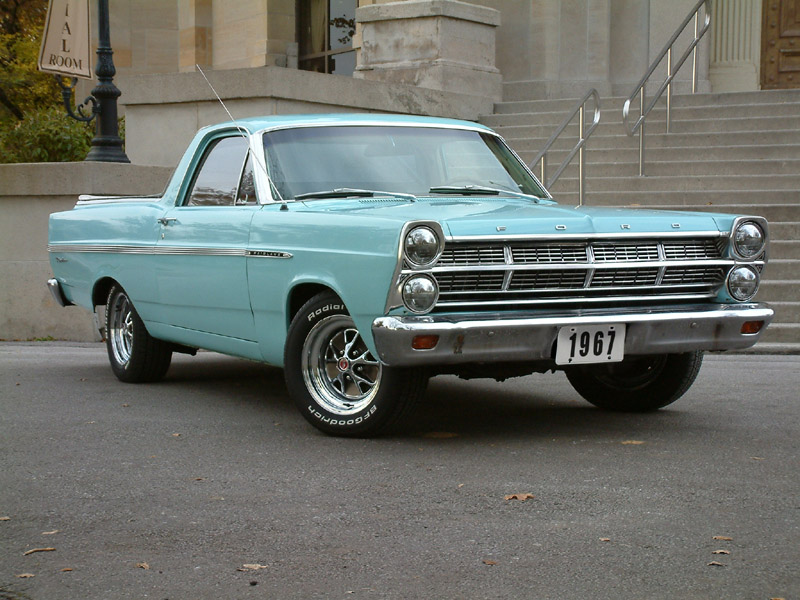
\includegraphics[height=0.8\textheight]{figures/1967_Ford_Fairlane_Ranchero.jpg}
\end{center}

\vfill
\tiny{\url{http://upload.wikimedia.org/wikipedia/commons/f/f5/1967_Ford_Fairlane_Ranchero.jpg}}

\end{frame}
%%%%%%%%%%%%%%%%%%%%%%%%%%%
\begin{frame}

\begin{center}
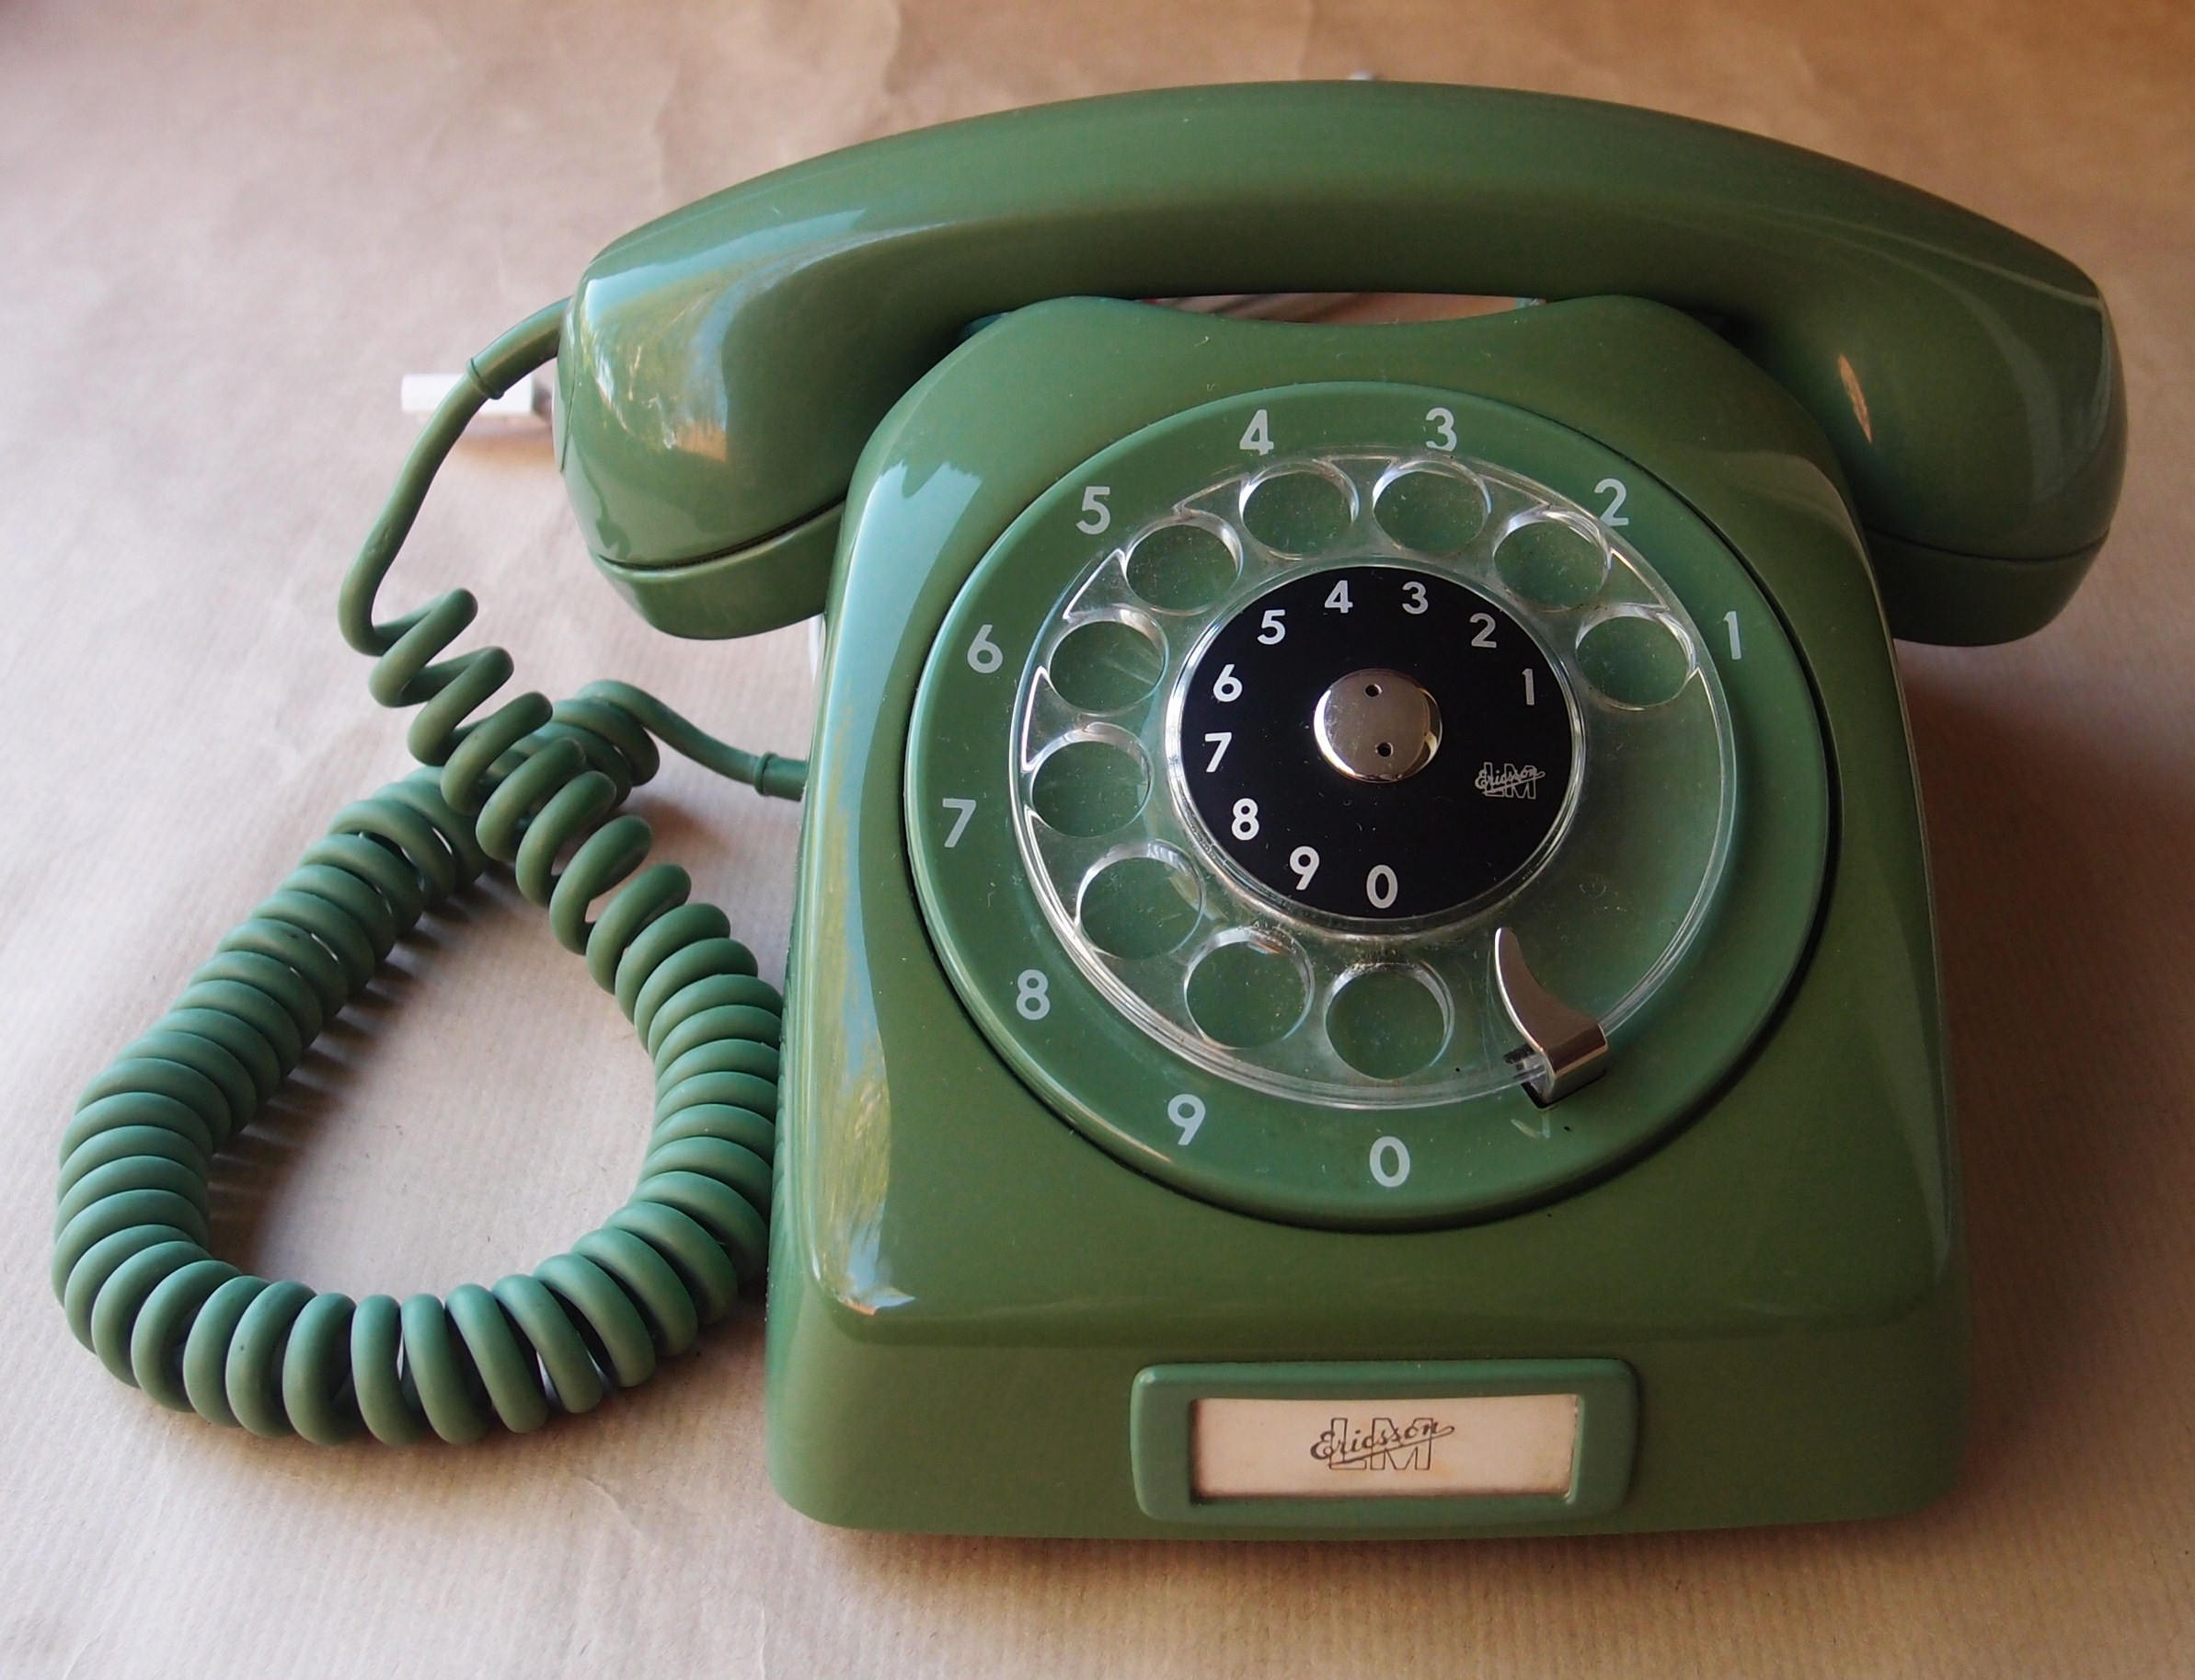
\includegraphics[height=0.8\textheight]{figures/Ericsson_Dialog_in_green}
\end{center}

\vfill
\tiny{\url{http://commons.wikimedia.org/wiki/File:Ericsson_Dialog_in_green.JPG}}

\end{frame}
%%%%%%%%%%%%%%%%%%%%%%%%%%%
\begin{frame}

\begin{center}
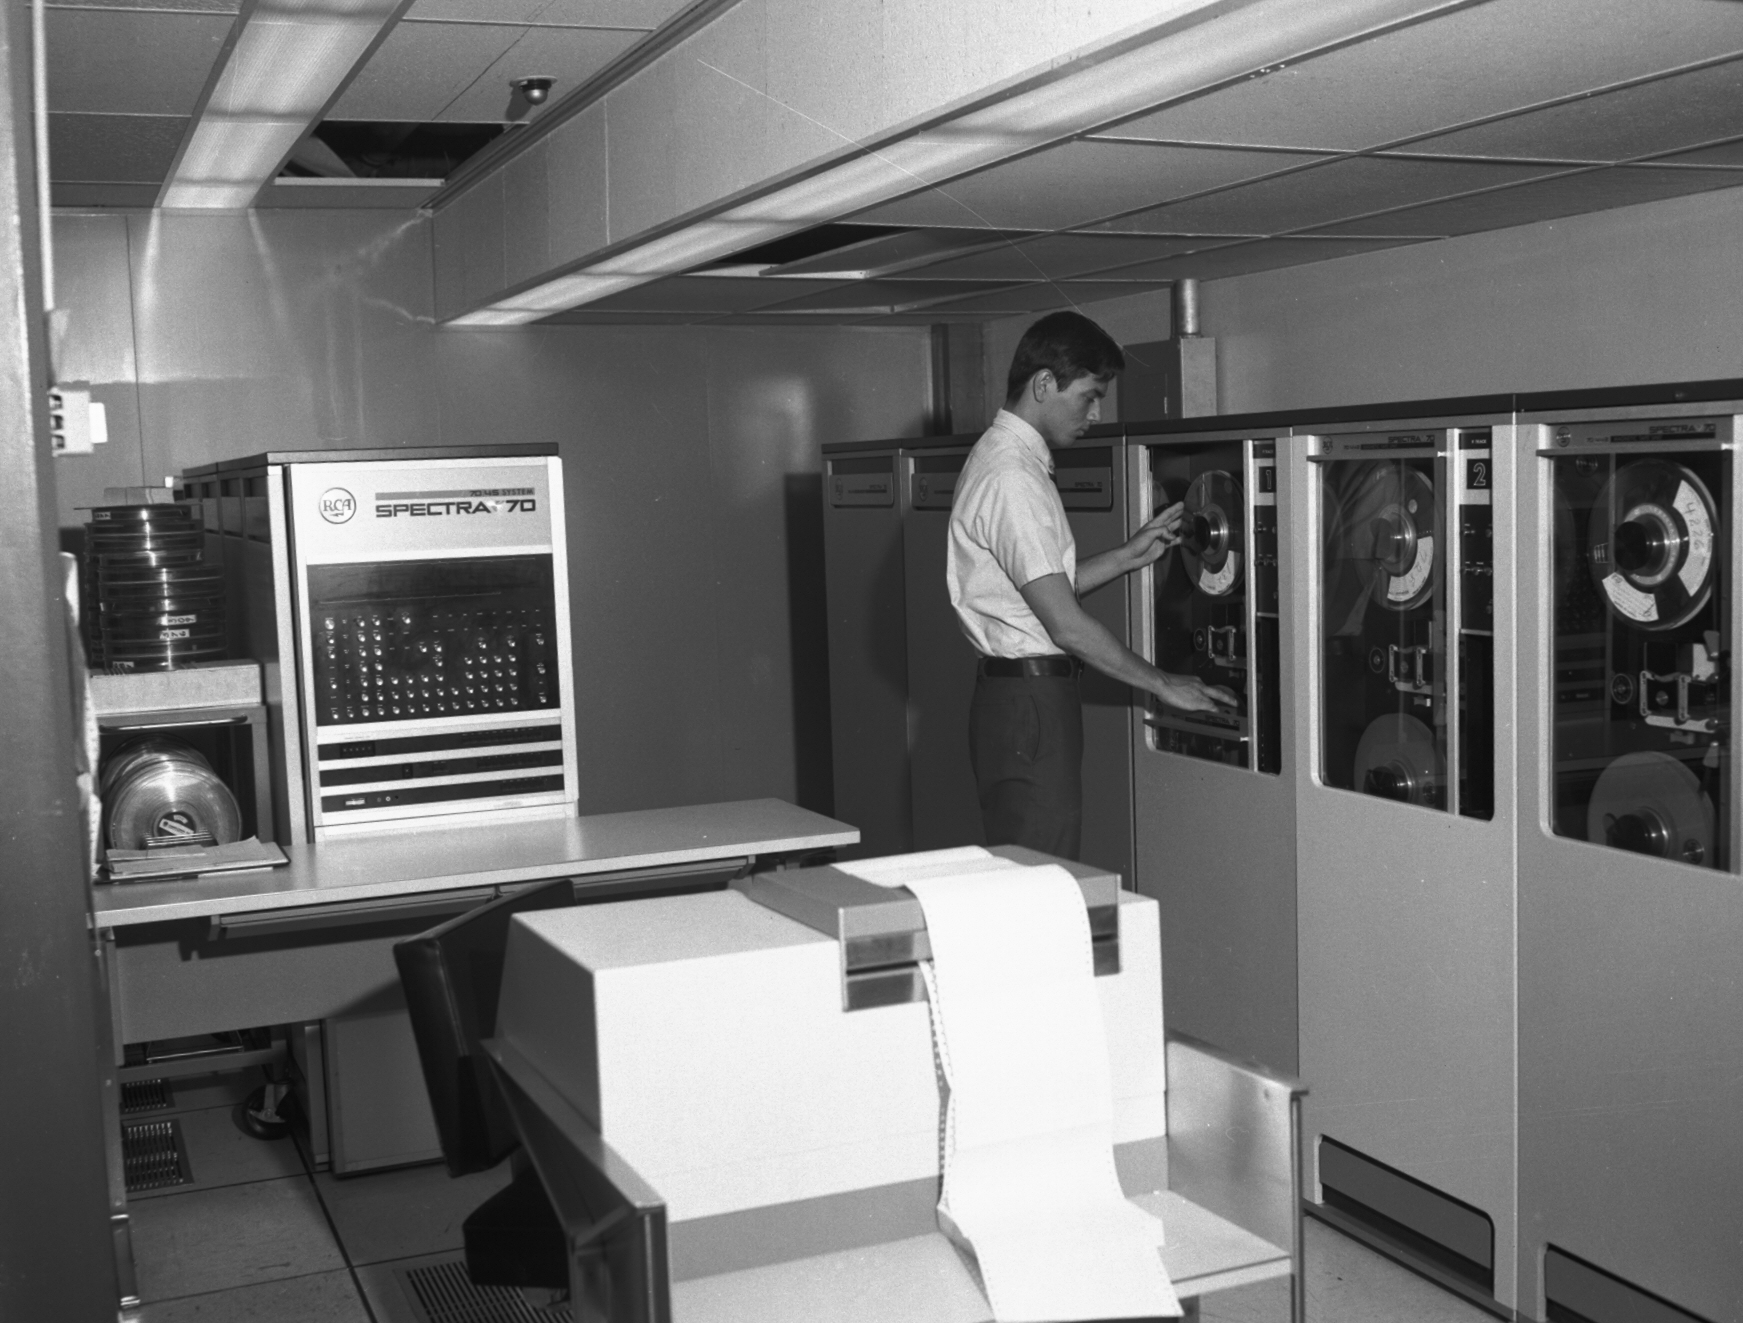
\includegraphics[height=0.8\textheight]{figures/Computer_in_County_of_Orange_offices,_1967}
\end{center}

\vfill
\tiny{\url{http://commons.wikimedia.org/wiki/File:Computer_in_County_of_Orange_offices,_1967.jpg}}

\end{frame}
%%%%%%%%%%%%%%%%%%%%%%%%%%%
\begin{frame}

Story $\rightarrow$ problem statement

\end{frame}
%%%%%%%%%%%%%%%%%%%%%%%%%%%
\begin{frame}

Given two individuals selected randomly from the population, what is the probability that the minimum number of intermediaries required to link them is 0,1,2,...k?

\end{frame}
%%%%%%%%%%%%%%%%%%%%%%%%%%%
\begin{frame}

\begin{center}
\begin{columns}
\begin{column}{0.4\textwidth}
Empirical approach\\(Harvard approach)
\end{column}
\begin{column}{0.2\textwidth}
vs.
\end{column}
\begin{column}{0.4\textwidth}
Modeling approach\\(MIT approach)
\end{column}
\end{columns}
\end{center}

\pause
\vfill
Today
\begin{itemize}
\item see how Dodds, Muhamad, and Watts tried to improve the empirical approach
\item learn some background so that we can understand a modeling approach
\end{itemize}

\end{frame}
%%%%%%%%%%%%%%%%%%%%%%%%%%%
\begin{frame}

``I read somewhere that everybody on the planet is separated by only six other people.  Six degrees of separation.  Between us and everybody else on this planet.  The president of the United States.  A gondolier in Venice . . . It's not just the big names.  It's anyone.  A native in the rain forest.  A Tierra del Fuegan.  An Eskimo.  I am bound to everyone on this planet by a trail of six people.  It's a profound thought . . . ''\\
Ouisa in \textit{Six Degrees of Separation} by John Guare (1990)

\pause
\vfill
science $\rightarrow$ art $\rightarrow$ science
 
\note{
Dodds et al read all the paper and they were probably also influenced by Guare
Milgram talks about 200 million americas
Guare scales it up to the world
Scientists try to test this literary idea
Science inspires art inspires science
}

\end{frame}
%%%%%%%%%%%%%%%%%%%%%%%%%%%%%
\begin{frame}

{\Large
\begin{center}
Analog vs Digital
\end{center}}

\end{frame}
%%%%%%%%%%%%%%%%%%%%%%%%%%%
\begin{frame}

Digital enables:
\begin{itemize}
\item zero-marginal cost data
\end{itemize}

\end{frame}
%%%%%%%%%%%%%%%%%%%%%%%%%%%%
\begin{frame}

\begin{center}
\includegraphics<1>[height = 0.95\textheight]{figures/zero_variable_cost_1}
\includegraphics<2>[height = 0.95\textheight]{figures/zero_variable_cost_2}
\end{center}

\note{
talk about scaling in each study
}

\end{frame}
%%%%%%%%%%%%%%%%%%%%%%%%%%%%
\begin{frame}

Digital enables:
\begin{itemize}
\item zero-marginal cost data
\item 100x'ing the number of participants
\pause
\item global scale
\end{itemize}

\pause
\vfill For more: Salganik (2018) \textit{Bit by Bit: Social Research in the Digital Age}: \url{http://www.bitbybitbook.com}

\note{
Global scale: imagine all the stamps and logistics
}

\end{frame}
%%%%%%%%%%%%%%%%%%%%%%%%%%%%
\begin{frame}

\begin{itemize}
\item What was the limiting factor for Travers and Milgram?
\item What was the limiting factor for Dodds, Muhamad, and Watts?
\end{itemize}

\note{
Travers and Milgram: Money
Dodds et al: attention
}

\end{frame}
%%%%%%%%%%%%%%%%%%%%%%%%%%%
\begin{frame}

24,163 chains started toward 18 targets all over the world.  The first time ever we have an experiment like this on a global scale.  What did they find?  

\note{The biggest study ever, years of coding in the basement, what did they find?}

\end{frame}
%%%%%%%%%%%%%%%%%%%%%%%%%%%%
\begin{frame}

\begin{center}
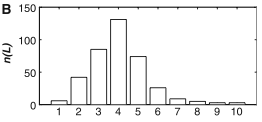
\includegraphics[width = 0.95\textwidth]{figures/dodds_experimental_2003_fig2b}
\end{center}

\vfill
$L =$ chain length (number of edges), mean of about 4

\note{Mean of 4 intermediaries, but remember this data is misleading because of attrition.  Think back to the coin flipping experiment.}

\end{frame}
%%%%%%%%%%%%%%%%%%%%%%%%%%%
\begin{frame}

\begin{center}
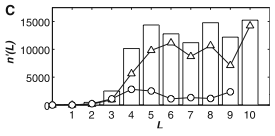
\includegraphics[width = 0.95\textwidth]{figures/dodds_experimental_2003_fig2c}
\end{center}

\vfill
Median of 5 (same country) to 7 (different country) intermediaries

\note{Median of 5 - 7 intermediaries}

\end{frame}
%%%%%%%%%%%%%%%%%%%%%%%%%%%
\begin{frame}

How did people decide who to pass the message to?\\

Location and occupation accounted for about half of all choices

\note{
This tells us something about people think the world is organized
}

\end{frame}
%%%%%%%%%%%%%%%%%%%%%%%%%%%
\begin{frame}

What was the chain completion rate for Dodds, Muhamad, and Watts?

\end{frame}
%%%%%%%%%%%%%%%%%%%%%%%%%%%
\begin{frame}

\begin{center}
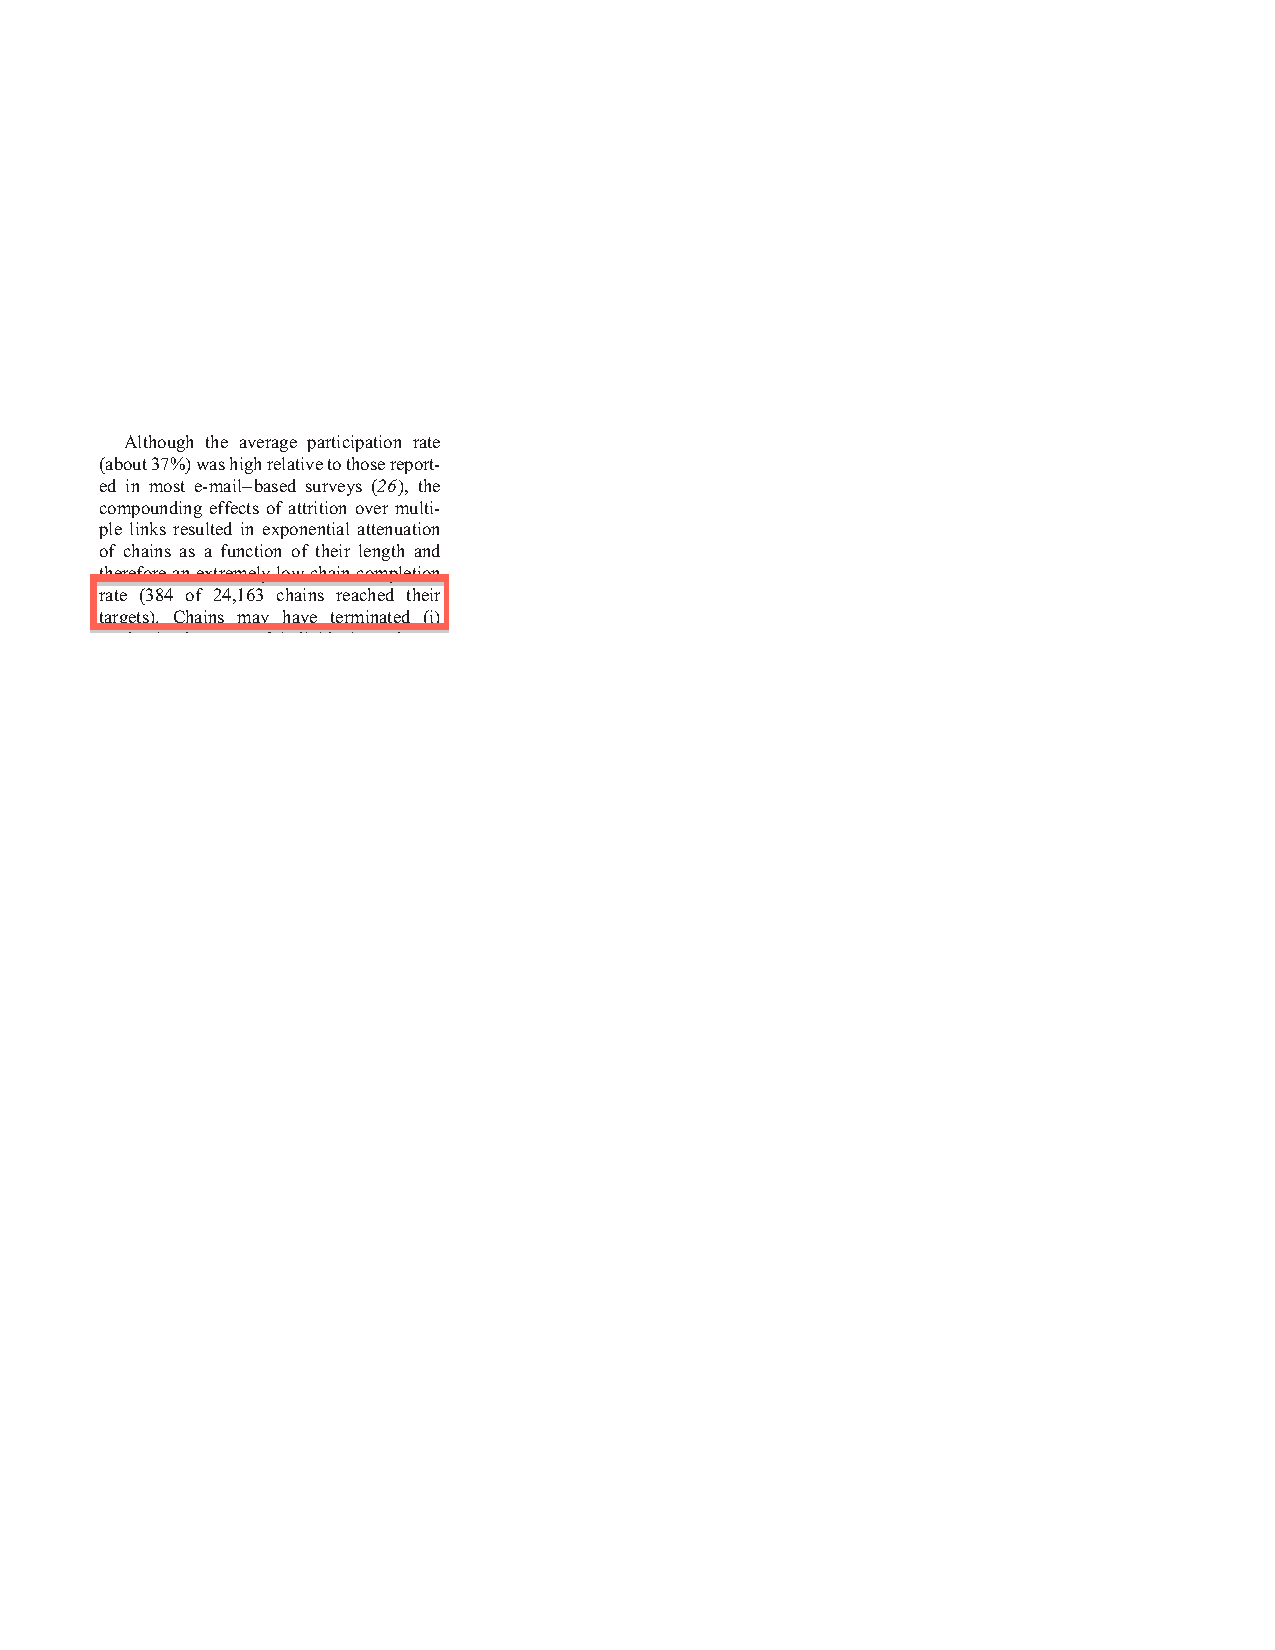
\includegraphics[width=0.9\textwidth]{figures/dodds_experimental_2003_completion}
\end{center}
\begin{center}
\LARGE{
$\frac{384}{24,163}= \textcolor{blue}{1.6\%}$
}
\end{center}

\note{24,163 initiated only 384 completed (that's 1.6\%)  98.4\% didn't complete.  Notice that the number 1.6\% is not in the paper anywhere, 98.4\% certainly not.  

Why is this important. The actual number is not important, but this is an important lesson in how to be an alert reader.   See who gets candy.

Like a magician: look over here and not over here
}

\end{frame}
%%%%%%%%%%%%%%%%%%%%%%%%%%%
\begin{frame}

Let's see what you all thought. . . .

\end{frame}
%%%%%%%%%%%%%%%%%%%%%%%%%%%
\begin{frame}


\begin{center}
\begin{columns}
\begin{column}{0.6\textwidth}
\begin{center}
\only<1>{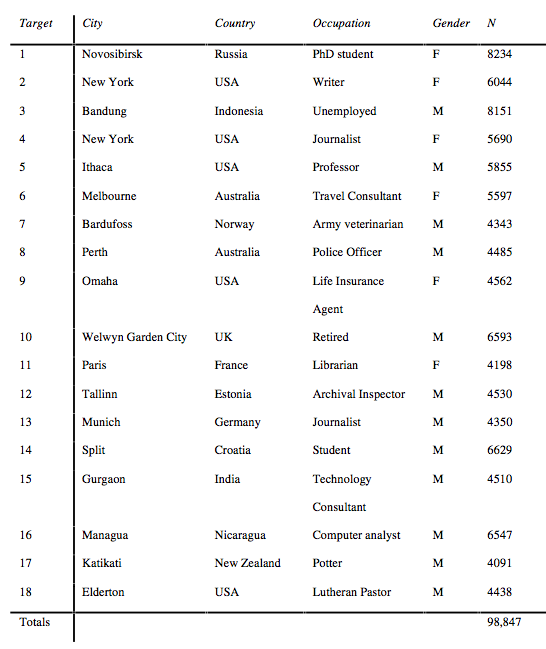
\includegraphics[height = 0.95\textheight]{figures/dodds_experimental_2003_tabS1_partial}}
\only<2-3>{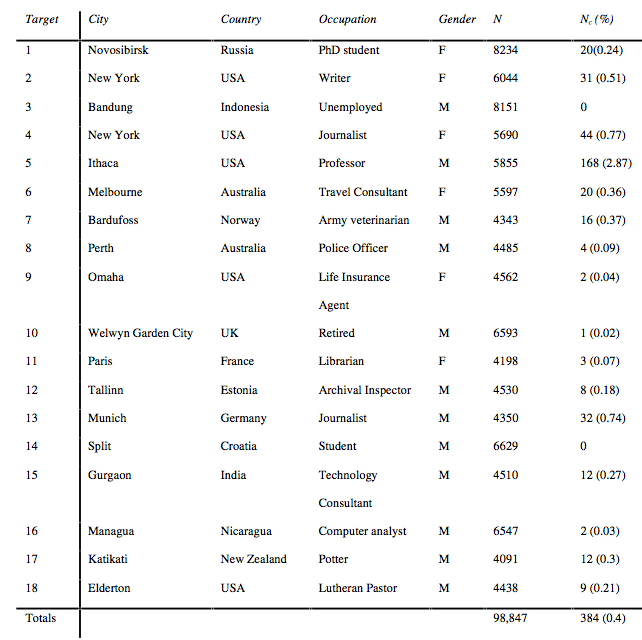
\includegraphics[height = 0.95\textheight]{figures/dodds_experimental_2003_tabS1_full}}
\end{center}
\end{column}
\begin{column}{0.01\textwidth}
\end{column}
\begin{column}{0.37\textwidth}
\begin{itemize}
\item Who had the lowest completion rate? \only<2>{unemployed person in Indonesia, student in Croatia. Note occupation is not a helpful dimension for these searches}
\item Who had the highest completion rate? \only<3>{Professor in Ithaca: Steve Strogatz and he's not that special (socially at least)} 
\end{itemize}
\end{column}
\end{columns}
\end{center}

\end{frame}
%%%%%%%%%%%%%%%%%%%%%%
\begin{frame}

\begin{itemize}
\item The largest empirical study of all time is mostly about connections to Steve Strogatz! (About 40\% of completed chains) \pause
\item Given two individuals selected randomly from the population, what is the probability that the minimum number of intermediaries required to link them is 0,1,2,...k? This is just a hard question to answer empirically.
\end{itemize}

\note{

This is just hard to study empirically.  Just like certain astronomical measurements are hard to make, this measurement is hard to make.  Meta note: When you are reading the papers, make sure not read them individually, but think about how they link together.  It seems like short chains may exist, but it is hard to collect data on them.  Recall that Milgram began his experiments because theoretical approaches were not working.  Here we have run into a data wall and now will go back to theory.

}

\end{frame}
%%%%%%%%%%%%%%%%%%%%%%%%%%%
\begin{frame}

What's next?

\end{frame}
%%%%%%%%%%%%%%%%%%%%%%%%%%%
\begin{frame}

\begin{center}
\begin{columns}
\begin{column}{0.4\textwidth}
Empirical approach\\(Harvard approach)
\end{column}
\begin{column}{0.2\textwidth}
vs.
\end{column}
\begin{column}{0.4\textwidth}
Modeling approach\\(MIT approach)
\end{column}
\end{columns}
\end{center}

\end{frame}
%%%%%%%%%%%%%%%%%%%%%%%%%%%
\begin{frame}

\begin{center}
\begin{columns}
\begin{column}{0.4\textwidth}
Empirical approach\\(Harvard approach)
\end{column}
\begin{column}{0.2\textwidth}
vs.
\end{column}
\begin{column}{0.4\textwidth}
\textcolor{blue}{Modeling approach\\(MIT approach)}
\end{column}
\end{columns}
\end{center}

\end{frame}
%%%%%%%%%%%%%%%%%%%%%
\begin{frame}

\begin{itemize}
\item What is the point of mathematical models?
\pause
\item How will we work with mathematical models in this class?
\end{itemize}

\note{
Billard balls, physics

}

\end{frame}
%%%%%%%%%%%%%%%%%%%%%%%%%%%
\begin{frame}

Erdos - Renyi Model

\note{
simplest possible model, draw a bunch of nodes on the board, throw down edges.  Giant component forms in a strange way

As you add edges the giant component does not grow linearly.  We will see things like this throughout the course: ice $\rightarrow$ water $\rightarrow$ steam

What is a mathematical model? Why is it useful?  When can it lead us astray?
}

\end{frame}
%%%%%%%%%%%%%%%%%%%%%%%%%%%
\begin{frame}

Demo

\vfill
\url{http://netlogoweb.org/launch\#http://netlogoweb.org/assets/modelslib/Sample\%20Models/Networks/Giant\%20Component.nlogo}
%\url{http://www.netlogoweb.org/launch\#http://ccl.northwestern.edu/netlogo/models/models/Sampl\%20Models/Networks/Giant\%20Component.nlogo}

\note{
run demo, with small number of nodes and watch giant component form, then reset with max number of nodes and re-run, but this time lets pretend these are Princeton students and the edges between then are sexual relationships.  If two people are not in the same component then they cannot spread STDs to each other.  
}

\end{frame}
%%%%%%%%%%%%%%%%%%%%%%%%%%%
\begin{frame}

We all get connected very quickly . . . 

\note{
Connection matters because things can spread
}

\end{frame}
%%%%%%%%%%%%%%%%%%%%%%%%%%%%
\begin{frame}

Is this is a good model for the social network at Princeton?\\
\pause
No. Not everyone is equally likely to be connected.

\end{frame}
%%%%%%%%%%%%%%%%%%%%%%%%%%%%
\begin{frame}

Network models
\begin{itemize}
\item Erdos-Reyni (dyadic)
\pause
\item Rappaport (triadic), wants the balance between randomness and order
\end{itemize}

\end{frame}
%%%%%%%%%%%%%%%%%%%%%%%%%%%
\begin{frame}

\begin{figure}
\centering
\includegraphics[width=\textwidth]{figures_book/2_3}
\end{figure}

\note{
Enter Rapoport\\
In Erdos-Reyni unit is dyad, Rapoport introduces the triad (Simmel said triads is where sociology begins)\\
Triadic closure bias a - b - c implies c - a (random biased nets)\\
Allows network to evolve over time, but runs into data and computing problems\\
How do you start? with random graph and fill in edges?  leads to completely connected network.  Duncan and I worked on this problem for one whole summer and got nowhere.\\

Point out difference between\\
\begin{itemize}
\item dynamics of networks
\item dynamics on networks
\end{itemize}

}

\end{frame}
%%%%%%%%%%%%%%%%%%%%%%%%%%%%
\begin{frame}

\begin{columns}
\begin{column}{0.6\textwidth}
For a detailed mathematical treatment of random graphs, I recommend:
\end{column}
\begin{column}{0.4\textwidth}
\begin{figure}
\centering
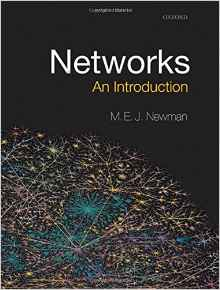
\includegraphics[width=\textwidth]{figures/newman_networks_2010_cover}
\end{figure}
\end{column}
\end{columns}

\end{frame}
%%%%%%%%%%%%%%%%%%%%%%%%%%%%%%%
\begin{frame}

\begin{figure}
\centering
\includegraphics[width=\textwidth]{figures/2_3}
\end{figure}

\note{
Graphs grow over time through triadic closure
}

\end{frame}
%%%%%%%%%%%%%%%%%%%%%%%%%%%%
\begin{frame}

\begin{figure}
\centering
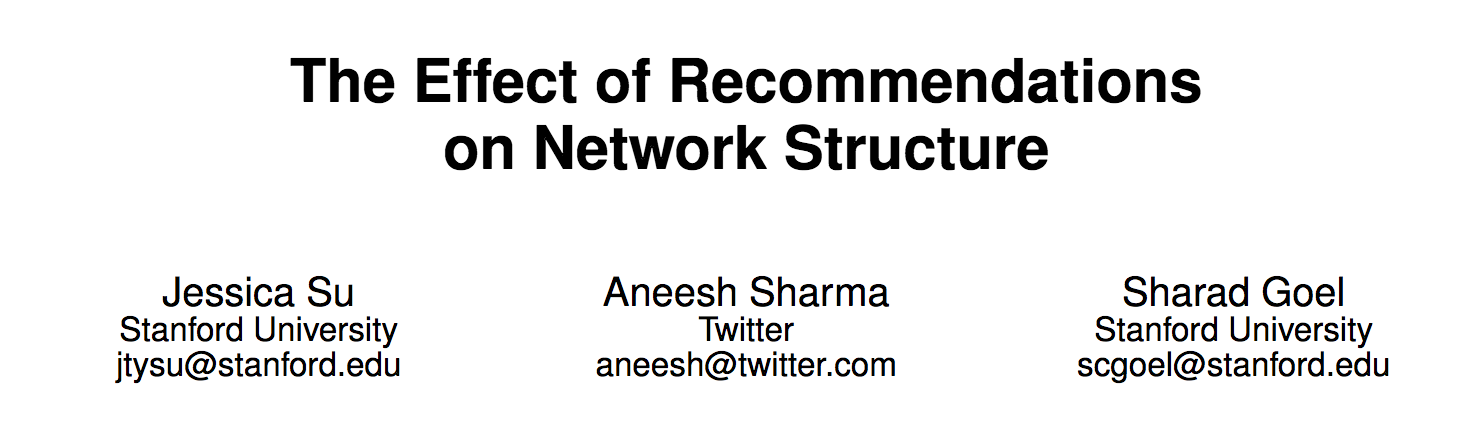
\includegraphics[width = \textwidth]{figures/su_effect_2016_title}
\end{figure}

\vfill

\url{http://dx.doi.org/10.1145/2872427.2883040}

\end{frame}
%%%%%%%%%%%%%%%%%%%%%%%%%%%%
\begin{frame}

\begin{figure}
\centering
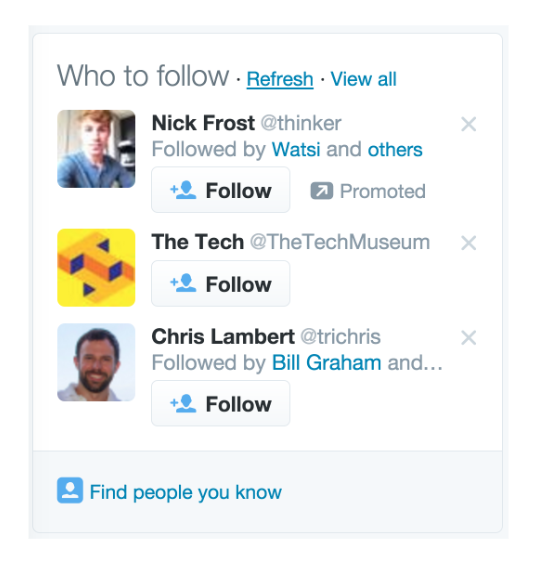
\includegraphics[height = \textheight]{figures/su_effect_2016_fig1}
\end{figure}

\end{frame}
%%%%%%%%%%%%%%%%%%%%%%%%%%%%
\begin{frame}

\begin{figure}
\centering
\includegraphics<1>[width = 0.3\textwidth]{figures/friend-of-friend-twitter_1}
\includegraphics<2>[width = 0.6\textwidth]{figures/friend-of-friend-twitter_2}
\includegraphics<3>[width = 0.6\textwidth]{figures/friend-of-friend-twitter_3}
\end{figure}


\note{
The people that the people you follow follow
Random walk to a person you follow then random walk to that person 
Good properties:
Easy computationally
More likely to recommend people more of your followers follow
}

\end{frame}
%%%%%%%%%%%%%%%%%%%%%%%%%%%%
\begin{frame}

\begin{figure}
\centering
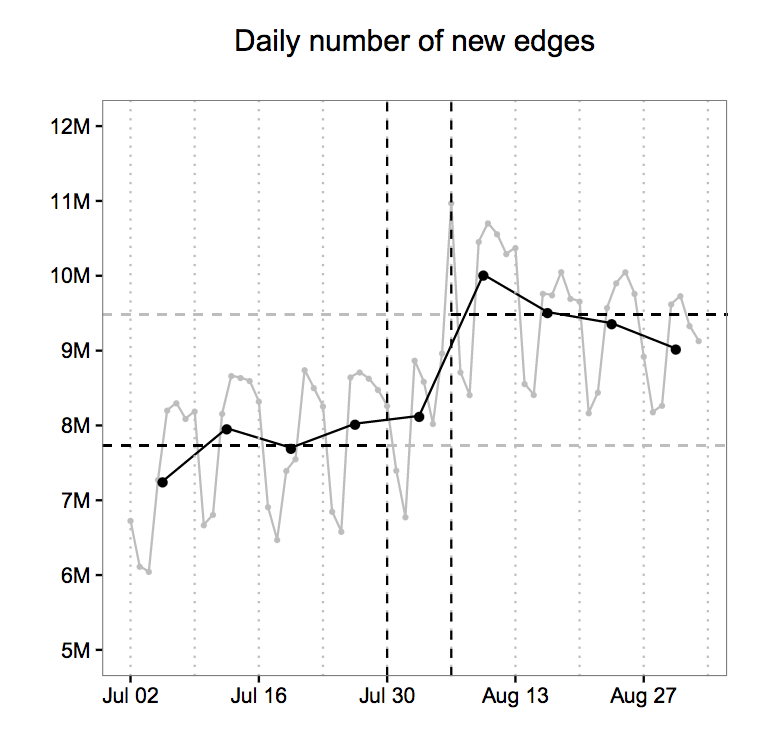
\includegraphics[height = \textheight]{figures/su_effect_2016_fig2}
\end{figure}

\end{frame}
%%%%%%%%%%%%%%%%%%%%%%%%%%%%
\begin{frame}

\begin{figure}
\centering
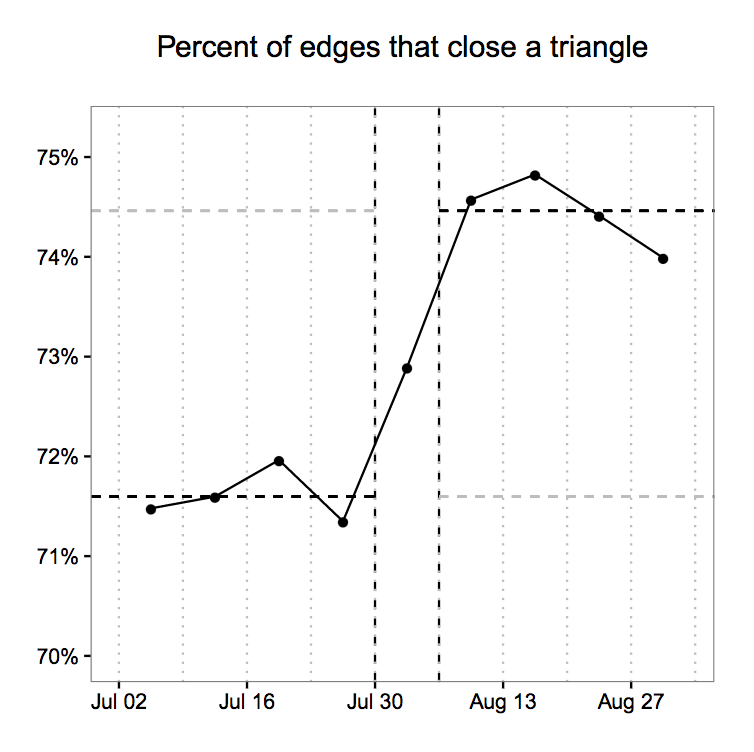
\includegraphics[height = \textheight]{figures/su_effect_2016_fig10a}
\end{figure}

\end{frame}
%%%%%%%%%%%%%%%%%%%%%%%%%%%%
\begin{frame}

Online behavior = human behavior + algorithmic bias

\note{
People who work at Facebook and Twitter took classes like this one
They have to solve problems so they bake in these ideas
}

\end{frame}
%%%%%%%%%%%%%%%%%%%%%%%%%%%%
\begin{frame}

Next class:\\
\pause
\begin{itemize}
\item Watts, Chapter 3.
\item Watts, D.J. and Strogatz, S.H. (1998). Collective dynamics of 'small-world' networks. \textit{Nature} 393, 440-442.
\item Victor, B. (2011). Scientific Communication As Sequential Art.
\item Watts, D.J. (1999). Networks, dynamics, and the small world phenomenon. \textit{American Journal of Sociology}, 105(2):493-527
\end{itemize}

\end{frame}
%%%%%%%%%%%%%%%%%%%%%%%%%%%
\begin{frame}

Feedback:\\
\Large{\url{http://bit.ly/soc204-2021}}

\end{frame}
%%%%%%%%%%%%%%%%%%%%%%%%%%%%


\end{document}
